\documentclass[11pt, handout]{beamer}

\usetheme{Darmstadt}
\usefonttheme{structurebold}
\setbeamertemplate{navigation symbols}{}

\usepackage{amsmath, amssymb}
\usepackage{tikz, braids}

\theoremstyle{example}
\newtheorem{goal}{Goal}

\title{Knotted Surfaces in Dimension Four}
\subtitle{Polymath}
%\author{Ana Wright}

\date{\small{August 15, 2021}}

\AtBeginSection[]{
  \frame{
  \vfill
  \centering
  \begin{beamercolorbox}[sep=8pt,center,shadow=true,rounded=true]{title}
    \usebeamerfont{title}\insertsectionhead\par%
  \end{beamercolorbox}
  \vfill
  }
}

\begin{document}
\frame{\titlepage}
\frame{
    \frametitle{Outline}
    \tableofcontents
}


%Isaiah's Notes:
%Introductory stuff: What is a knotted/unknotted surface surface
%Give simplest diagrams
%Introduce tri-plane moves
%Introduce invariants
%Connected Sum


\section{Introduction}

\frame{\frametitle{Unknots and Unlinks}
What is a knotted surface? We must first start with some general knot theory. 

\begin{definition}
The \textit{unknot} is the simplest knot, defined as an unknotted circle (or something isotopic) which lies in $\mathbb{R}^3.$
\end{definition}

\begin{definition}
A \textit{$c$-component unlink} is a diagram which can be untangled into $c$ copies of the unknot.
\end{definition}

}

\frame{\frametitle{Tri-plane Diagrams}
We can give a two-dimensional representation of a surface $K$ in $\mathbb{R}^4$ via a \textit{tri-plane diagram} [c.f. Figure: 1].

\begin{figure}
    \centering
    \includegraphics[scale= .3]{fig_1.jpg}
    \caption{1. An example of a tri-plane diagram $K=(K_1,K_2,K_3).$}
    \label{fig:my_label}
\end{figure}

A valid tri-plane diagram must satisfy:
\begin{itemize}
    \item Should have the same number of strands (and hence same number of endpoints on the horizontal axis).
    
    \item Each strand should be a trivial tangle, that is, each strand has one relative maximum w.r.t the horizontal axis.
    
    \item Each of $K_1\cup\overline{K_2},$ $K_2\cup\overline{K_3},$ and $K_3\cup\overline{K_1}$ should be diagrams for an unlink.
\end{itemize}
}

\frame{\frametitle{Tri-plane Diagrams (continued)}

One can verify that the diagram in Figure: 1 is a tri-plane diagram. In fact, it depicts the knotted surface known as the spun trefoil.

\medskip
Clearly, each tangle is trivial and each diagram has four strands. Inspecting the below figure allows us to verify that each mirrored union is an unlink.

\begin{figure}
    \centering
    \includegraphics[scale=.5]{fig_2.jpg}
    \caption{2. A verification that the mirrored unions are unlinks.}
    \label{fig:my_label}
\end{figure}


}

\frame{\frametitle{Tri-plane Moves}

Just as in $3$-dimensional knot theory, tri-plane diagrams can undergo local changes via the three Reidemeister moves, which are pictured in Figure 3.

\begin{figure}
    \centering
    \includegraphics[scale=.4]{reidemeister.jpg}
    \caption{3. The three Reidemeister moves.}
    \label{fig:my_label}
\end{figure}

Additionally, we can perform mutual braid moves, which are shown in Figure 4.

\begin{figure}
    \centering
    \includegraphics[scale=.4]{braid.jpg}
    \caption{4. A mutual Braid Move}
    \label{fig:my_label}
\end{figure}


}

\frame{\frametitle{Tri-plane moves (continued)}

We can also perform stabilization and destabilization moves as pictured in Figure 5.

\begin{figure}
    \centering
    \includegraphics[scale=.4]{stab.jpg}
    \caption{5. Stabilization and Destabilization}
    \label{fig:my_label}
\end{figure}

\begin{definition}
A \textit{tri-plane move} is either a Reidemeister move, a mutual braid move, or a stabilization/destabilization. 
\end{definition}



}

\frame{
    \frametitle{Tri-plane Diagrams for Unknotted Surfaces}
    \begin{itemize}
        \item Diagram for $P^{+}$
        \begin{figure}
        \centering
        \includegraphics[scale= .08]{P+.jpg}
        \end{figure}
        \item Diagram for $P^{-}$
        \begin{figure}
        \centering
        \includegraphics[scale= .08]{P-.jpg}
        \end{figure}
        \item Diagram for $T$
        \begin{figure}
        \centering
        \includegraphics[scale= .08]{T.jpg}
        \end{figure}
        \item Diagram for $U$
        \begin{figure}
        \centering
        \includegraphics[scale= .08]{U.jpg}
        \end{figure}
    \end{itemize}
}
\frame{\frametitle{Knotted Surfaces}

    \frametitle{Unknotted Surfaces}
    \begin{itemize}
        \item We write $K\sim K'$ if $K'$ can be obtained from $K$ via a finite series of tri-plane moves and planar isotopies.
        One can check that $\sim$ as defined above is an equivalence relation with equivalence class $[K].$ We call $[K]$ a \textit{knotted surface.} 
        \item We call a surface \textit{unknotted} if it is either the unknotted two-sphere U, or a finite connected sum of copies of the positive unknotted projective plane $P^{+}$, the negative unknotted projective plane $P^{-}$, or the unknotted torus, $T$.
    \end{itemize}
}
\frame{\frametitle{Writhe}
\begin{definition}

Take a knot (or link) diagram and assign an orientation by moving along the knot with arrows. To each crossing where the arrow in the right direction is an over crossing, associate a $+1.$ To each crossing where the arrow pointing right is an under crossing, associate a $-1.$ We define the \textit{writhe} of $K,$ $w(K)$ as the sum of these $+1$ and $-1$ which appear at each crossing.
\end{definition}

\begin{figure}
    \centering
    \includegraphics[scale=.3]{writhe.jpg}
    \caption{6. Computing Writhe}
    \label{fig:my_label}
\end{figure}


}


\frame{\frametitle{Bridge Number and Crossing Number}

\begin{definition}
We define the \textit{bridge number} $b(K)$ of a tri-plane diagram $K$ as the number of strands in each picture. The bridge number of an unknotted surface $b([K])$ is defined to be the minimal bridge number that appears for the given surface, i.e.
$b([K]) = \min\{b(K')\,:\, K\sim K'\}.$
\end{definition}

\begin{definition}
We define the \textit{crossing number} $c(K)$ of a tri-plane diagram $K$ is the number of times that strands in all three diagrams cross. The crossing number of a knotted surface $c([K])$ is defined as the minimal crossing number that appears in some representation of the surface $K,$ i.e.e $c([K])=\min\{c(K')\,:\,K'\sim K\}.$
\end{definition}



}

\frame{\frametitle{Patch Numbers and Invariants}
\begin{definition}
We define the \textit{patch numbers} $p_{12},$ $p_{23},$ and $p_{31}$ as the number of components which appear in the unlinks for $K_1\cup \overline{K_2},$ $K_2\cup \overline{K_3},$ and $K_3\cup \overline{K_1},$ respectively.
\end{definition}

\begin{definition}
We define the\textit{ Euler characteristic} of a surface $K$ as $\chi(K) = p_{12}+p_{23}+p_{31}-b,$ where $p_{ij}$ are the patch numbers and $b$ is the bridge number. We call $\chi$ an invariant because if $K\sim K',$ then $\chi(K)=\chi(K').$
\end{definition}

\begin{definition}
We define the \textit{normal Euler number} of a surface $K$ as $e(K)= w(K_1\cup \overline{K_2})+w(K_2\cup \overline{K_3})+w(K_3\cup\overline{K_1}).$ We call $e$ and invariant because if $K\sim K',$ then $e(K)=e(K').$
\end{definition}
}



\frame{\frametitle{Orientability}
\begin{definition}
Given a tri-plane diagram $K$ with $b$ strands, to each endpoint we will associate either a $+$ or a $-.$ We do so in such a way so that each strand has a $+$ at one endpoint and a $-$ at the other. We also ensure that the signs are consistent between all three diagrams. If all $2b$ signs in each diagram match and each strand receives one sign each, then we say that $K$ is \textit{orientable,} and we write $o(K)=1.$ Otherwise, $o(K)=0.$ It is worth noting that $o$ is also an invariant.
\end{definition}

\begin{figure}
    \centering
    \includegraphics[scale=.3]{orientable_trefoil.jpg}
    \caption{7. The spun trefoil is orientable.}
    \label{fig:my_label}
\end{figure}

}

\frame{\frametitle{Connected Sums}

Another definition: 

\begin{definition}
Consider two tangle diagrams $K_1$ and $K_2.$ We can take a connected sum $K_1\#K_2$ of the diagrams by detaching an endpoint on each diagram from the $y$-axis and connecting them. See the below figure.

\begin{figure}
    \centering
    \includegraphics[scale=.5]{connected_sum.jpg}
    \caption{8. Connected sum of two tangle diagrams.}
    \label{fig:my_label}
\end{figure}

\end{definition}



}

\section{Group G's Work}
\frame{
    \frametitle{Representing Tangles}
    \begin{itemize}
        \item Need to tell a computer what a tangle is
        \pause
        \item Snappy/Spherogram are good, but not what we need
        \pause
        \item Idea: a trivial tangle is a \emph{braid} plus a \emph{cap diagram}
        \pause
        \item Braids: form a group; Sage understands this group
			\medskip
            	\begin{center}
            		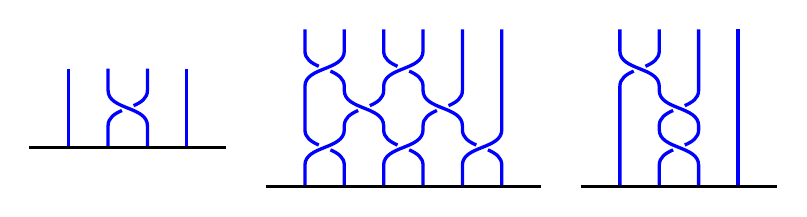
\begin{tikzpicture}
            			\braid[
            				number of strands=4,
            				very thick, blue,
            				width=0.5cm,
            				height=0.5cm,
            			] (b1) at (0,0) s_2;
            			\draw[very thick] (-0.5,-1) -- (2,-1);
            			
            			\braid[
            				number of strands=6,
            				very thick, blue,
            				width=0.5cm,
            				height=0.5cm
            			] (b2) at (3,0.5) s_1^{-1}-s_3^{-1} s_2-s_4 s_1^{-1}-s_3^{-1}-s_5^{-1};
            			\draw[very thick] (2.5,-1.5) -- (6,-1.5);
            			
            			\braid[
            				number of strands=4,
            				very thick, blue,
            				width=0.5cm,
            				height=0.5cm
            			] (b3) at (7,0.5) s_1 s_2 s_2;
            			\draw[very thick] (6.5,-1.5) -- (9,-1.5);
            		\end{tikzpicture}
            	\end{center}
    \end{itemize}
}

\frame{
    \frametitle{Representing Tangles}
    \begin{itemize}
        \item Cap diagram:
        		\begin{center}
        			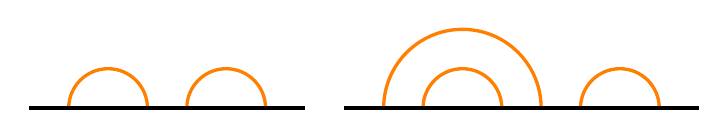
\begin{tikzpicture}
        				\draw[very thick, orange] (0,0) arc (180:0:0.5);
        				\draw[very thick, orange] (1.5,0) arc (180:0:0.5);
        				\draw[very thick] (-0.5,0) -- (3,0);
        				
        				\draw[very thick, orange] (4,0) arc (180:0:1);
        				\draw[very thick, orange] (4.5,0) arc (180:0:0.5);
        				\draw[very thick, orange] (6.5,0) arc (180:0:0.5);
        				\draw[very thick] (3.5,0) -- (8,0);
        			\end{tikzpicture}
        		\end{center}
        \pause
        \item Cap diagrams are generated using a classical algorithm
        \pause
        \item Capping off braids:
        		\begin{center}
        			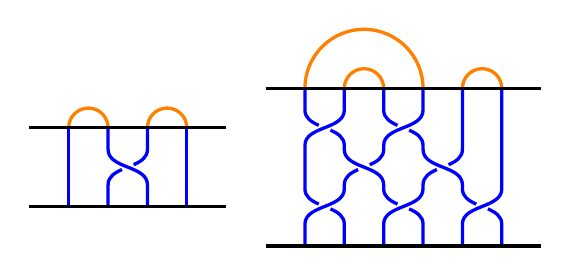
\begin{tikzpicture}
        				\braid[
            				number of strands=4,
            				very thick, blue,
            				width=0.5cm,
            				height=0.5cm,
            			] (b1) at (0,0) s_2;
            			\draw[very thick, orange] (b1-1-s) arc (180:0:0.25);
            			\draw[very thick, orange] (b1-3-s) arc (180:0:0.25);
            			\draw[very thick] (-0.5,-1) -- (2,-1);
            			\draw[very thick] (-0.5,0) -- (2,0);
            			
            			\braid[
            				number of strands=6,
            				very thick, blue,
            				width=0.5cm,
            				height=0.5cm
            			] (b2) at (3,0.5) s_1^{-1}-s_3^{-1} s_2-s_4 s_1^{-1}-s_3^{-1}-s_5^{-1};
            			\draw[very thick, orange] (b2-1-s) arc (180:0:0.75);
            			\draw[very thick, orange] (b2-2-s) arc (180:0:0.25);
            			\draw[very thick, orange] (b2-5-s) arc (180:0:0.25);
            			\draw[very thick] (2.5,-1.5) -- (6,-1.5);
            			\draw[very thick] (2.5,0.5) -- (6,0.5);
        			\end{tikzpicture}
        		\end{center}
    \end{itemize}
}

\frame{
    \frametitle{Listing Triplane Diagrams}
    \begin{goal}
        List all triplane diagrams with small bridge \& crossing \#.
    \end{goal}
    \pause
    \begin{itemize}
        \item How do we check if three trivial tangles form a triplane diagram?
            \begin{enumerate}
                \item Translate to Spherogram
                \item Check if resulting links are unlinks
            \end{enumerate}
        \pause
        \item Problem: this takes a \emph{really} long time
            \begin{itemize}
                \item There are A LOT of braids
                \item Looking at three tangles cubes everything
            \end{itemize}
        \pause
        \item Solutions:
            \begin{itemize}
                \item Braids are words in generators, so remove duplicates
                \item Generation and verification separately
            \end{itemize}
    \end{itemize}
}

\frame{
    \frametitle{Computing Invariants}
    \begin{goal}
        Automatically compute invariants of a triplane diagram
    \end{goal}
    \pause
    \begin{itemize}
        \item Orientability and Euler characteristic: variations on greedy algorithm
            \begin{itemize}
                \item Start at an arbitrary point/orientation
                \item Chase around the diagrams making inferences
            \end{itemize}
        \pause
        \bigskip
        \item Other invariants: Snappy/Spherogram
            \begin{itemize}
                \item E.g., computing writhe
            \end{itemize}
    \end{itemize}
}


% Yucong's notes
% 1.
% Section for crossing numbers of unknotted surfaces
% definition of unknotted surface
% diagrams for U,T,P+,P-
% categorize into orientable (in the form of T^n) and non-orientable surfaces (in the form of P^{n,m})
% 2.
% prelimiary inequality for crossing numbers of unknotted surfaces
% diagrams for unions of tangles
% |n-m|\leq c(P^{n,m})\leq max(n,m)
% 3.
% main result: c(P^{n,m}) = max(1, |n-m|)
% Mirror Property: P{n,m} = P{m,n}
% 4.
% tri-plane moves for minimum crossing of P{n,n}, P{n,n+1}
% diagrams for tri-plane moves
% use the results of P{n,n}, P{n,n+1} to bound the crossing numbers of all other P{n,m}:  (m-n-1)(0,1) + (n,n+1) = (n,m), m > n 
% (?) crossing number = 1 , 2 => unknotted
% open problems: moves for cap-braid diagram catagory;  
\section{Group O2's Work}

\frame{
    \frametitle{Some Preliminary Results}
    \begin{itemize}
        \item \textbf{Proposition 1} $[T\#P^{+}] = [P^{+}\#P^{-}\#P^{+}]$,$[T\#P^{-}] = [P^{-}\#P^{+}\#P^{-}]$
        \item \textbf{Remark} If an unknotted P is orientable, then $[P] = [U]$ or $[P] = [T^n]$; otherwise $[P] = [P^{+}]^{n}\#[P^{-}]^{m}=: P^{n,m}$.
        \item \textbf{Proposition 2} For any tri-plane diagram $P$, $|e(P)|\leq 2c(P)$.
        \item \textbf{Corollary 3} $|n-m| \leq c(P^{n,m})\leq max\{n,m\}$.
        \item \textbf{Proposition 4} $c([P\# P']) \leq c([P]) + c([P'])$.
        \item \textbf{Proposition 5} If $c([P]) = 0$, then $[P]$ is orientable.
    \end{itemize}
}
\frame{
    \frametitle{Main Results}
    \begin{theorem}
    $c([P^{n,m}]) = max\{1,|n-m|\}$
    \end{theorem}
    \begin{proof}
        \begin{itemize}
            \item \textbf{Step I.} Prove $c([P^{n,m}]) = c([P^{m,n}])$
            \item \textbf{Step II.} Prove $c([P^{n,n}]) = c([P^{n,n+1}]) = 1$
            \item \textbf{Step III.} Apply Prop. 4: $c([P^{n,n + k}]) \leq c([P^{n,n+1}]) + (k-1)c([P^{0,1}])= 1 + (k-1) = k$
        \end{itemize}
    \end{proof}
}
\frame{
    \frametitle{Step II}
    \begin{lemma}
        $\forall n\in \mathbb{N}_{+}, [P^{n,n}]$ has a diagram that looks like the following: 
        \begin{figure}
        \centering
        \includegraphics[scale= .07]{tri_pnn.jpg}
        \end{figure}
    \end{lemma}
    \begin{itemize}
        \item We use the pair of unlink diagrams, $P_{12} = P_1\cup \overline{P_2}$ and $P_{32} = P_3\cup \overline{P_2}$ to visualize the tri-plane moves to reduce crossings.
        \begin{figure}
        \centering
        \includegraphics[scale= .08]{braid_move_glued.jpg}
        \end{figure}
    \end{itemize}
}
\frame{
    \frametitle{Step II}
    \begin{proof}
        \begin{itemize}
            \item Base case n = 1:
            \begin{figure}
            \centering
            \includegraphics[scale= .2]{base_case.jpg}
            \end{figure}
        \end{itemize}
    \end{proof}
}
\frame{
    \frametitle{Step II}
    \begin{proof}
        \begin{itemize}
            \item Inductive Step from $n$ to $n+1$:
            \begin{figure}
            \centering
            \includegraphics[scale= .08]{1st_move_pnn.jpg}
            \end{figure}
            \begin{figure}
            \centering
            \includegraphics[scale= .08]{2nd_move_pnn.jpg}
            \end{figure}
        \end{itemize}
    \end{proof}
}
\frame{
    \frametitle{Step II}
    \begin{corollary}
    $c([P^{n,n+1}]) = 1$
    \end{corollary}
    \begin{proof}
        \begin{itemize}
            \item Perform a left translation as follows \begin{figure}
            \centering
            \includegraphics[scale= .1]{move_pnn+1.jpg}
            \end{figure}
        \end{itemize}
    \end{proof}
}
\frame{
    \frametitle{Future Work}
    \begin{block}{Conjecture}
    If $c([P]) < 4$, then $[P]$ is unknotted.
    \end{block}
}

\section{Group O3's Work}
\frame{
    \frametitle{Goal: Compile a Body of Knotted Surfaces}
    \begin{itemize}
    \item <1-> Examples are immensely helpful in the research process as they build intuition and are critical for testing conjectures.
    \item <2-> In regular knot theory, it is easy to work with and come up with new knots. 
    \item <3-> Unfortunately, coming up with a list of distinct and interesting tri-plane diagrams for knotted surfaces is not easy.
    \end{itemize}}
\frame{
    \frametitle{CH-Diagrams}
    Luckily, there are already lists of knotted surfaces.
    \begin{columns}[t]
        \column{.4\textwidth}
        \centering
        \includegraphics[width=5cm,height=4cm]{ojm1.png}\\
        \column{.5\textwidth}
        \centering
        \includegraphics[width=5cm,height=4cm]{ojm2.png}\\
    \end{columns}
}
\frame{
    \frametitle{Converting CH-Diagrams}
    Here we see a ch-diagram and a tri-plane diagram for the spun trefoil knotted surface.\\
    \begin{columns}[t]
        \column{.3\textwidth}
        \includegraphics[width=3cm,height=3cm]{Spun-Trefoil.png}
        \column{.6\textwidth}
        \centering
        \includegraphics[width=7cm,height=2.5cm]{fig_1.jpg}
    \end{columns}
}
\frame{
    \frametitle{Converting CH-Diagrams}
    To convert a CH-diagram, we first want to put it into bridge position.\\
    \begin{columns}[t]
        \column{.2\textwidth}
        \includegraphics[width=3.5cm,height=3cm]{Spun-Trefoil_unlabeled.png}
        \column{.6\textwidth}
        \centering
        \includegraphics[width=6cm,height=3.5cm]{tre-bridge.png}
    \end{columns}
}

\frame{
    \frametitle{Converting CH-Diagrams}
    We then resolve the top portion into two tangles, and the bottom into it's own.\\
    \begin{columns}[t]
        \column{.2\textwidth}
        \includegraphics[width=3.5cm,height=3cm]{tre-bridge.png}
        \column{.6\textwidth}
        \centering
        \includegraphics[width=6cm,height=3.5cm]{Spun-Trefoil-Triplane.png}
    \end{columns}
}

\frame{
    \frametitle{Converting CH-Diagrams}
    \begin{itemize}
        \item <1> We then verify if the tangles make up a valid tri-plane diagram.
        \item <2> If they don't, we have to start over and try again with a different bridge position.
        \item <3> Once we have a tri-plane diagram we can calculate invariants for the diagram.
    \end{itemize}
}



\section{Conclusion}

\frame{
    \frametitle{Acknowledgements}
    \large
    Big thanks to\ldots\medskip
    \begin{itemize}
        \item Alex Zupan, Ana Wright, and Nick Meyer for guidance and insight
        \bigskip
        \item Polymath REU organizers for this wonderful opportunity!
    \end{itemize}
}

\frame {
\frametitle{References}
\bibliographystyle{amsplain}
\begin{thebibliography}{11}

\bibitem{MZ} J. Meier \& A. Zupan. Bridge trisections of knotted surfaces in $S^4$. 2017. \emph{Transactions of the American Mathematical Society} \textbf{369}, 7343-7386. \url{https://doi.org/10.1090/tran/6934}

\bibitem{Y} H. Yoshikawa. An enumeration of surfaces in four-space. 1994. Osaka Journal of Mathematics \textbf{31}(3): 497-522.

\end{thebibliography}
}

\end{document}